% Provenance (never printed): old premiere S material on plate kinematics (rigid
% plates, rates from magnetic anomalies and from satellite positioning, hotspots
% and the Hawaiian chain, the coherence of the model); see
% sources/book2/PROVENANCE.md. Velocities from the NNR-MORVEL56 poles
% (figdata/grade-11/plate_velocities.py), station series from the Nevada Geodetic
% Laboratory (gnss_series.py), volcano ages from Clague and Dalrymple 1987
% (hawaii_chain.py). Euler poles and triple junctions belong to Year 1: the
% rotation pole is told, not defined.
\chapter{As placas e os seus movimentos}\label{ch:g11:plate-motions}

Perto do cume do Mauna Kea, na ilha do Havaí, uma antena fixada na rocha
recebe todos os dias, desde outubro de 1996, os sinais dos satélites de
posicionamento. A cada dia, um computador calcula onde a antena está, com
precisão de poucos milímetros. Trinta anos de posições contam a mesma
história todos os anos: a antena, a montanha e a ilha inteira se deslocam
cerca de \qty{7}{cm} por ano em direção ao oés-noroeste, sem parar e sem
virar. Em 2026, a antena estava a mais de dois metros do ponto de partida.
Este capítulo mede esses movimentos, mostra como eles se encaixam sobre uma
esfera e lê o mesmo movimento na cadeia de vulcões extintos que se estende
do Havaí através do Pacífico Norte.
% ledger: data:b2-ngl-gnss

\begin{recall}
A \omterm{def:g11:lithosphere-asthenosphere:lithosphere}{litosfera} é dividida em placas tectônicas que se movem umas em relação às
outras a alguns centímetros por ano; os seus limites são dorsais, fossas,
zonas de colisão e falhas transformantes (Livro 1, 7º ano). Um ponto quente
é um lugar no fundo do manto que alimenta um vulcão na placa acima dele; a
placa leva o vulcão embora enquanto um novo cresce sobre o ponto quente
(Livro 1, 7º ano). Um receptor de posicionamento por satélite calcula a sua
própria posição a partir dos sinais de vários satélites (Livro 1, 9º ano).
As listras magnéticas do fundo do oceano dão a \omterm{def:g11:drift-to-spreading:spreading-rate}{taxa de expansão} de uma
dorsal (\cref{ch:g11:drift-to-spreading}), e a \omterm{def:g11:lithosphere-asthenosphere:lithosphere}{litosfera} é a camada externa
rígida da Terra, com cerca de \qty{100}{km} de espessura
(\cref{ch:g11:lithosphere-asthenosphere}). Uma velocidade de \qty{1}{cm} por
ano equivale a \qty{10}{km} por milhão de anos, e \qty{1}{mm} por ano a
\qty{1}{km} por milhão de anos.
\end{recall}

\begin{omfigure}
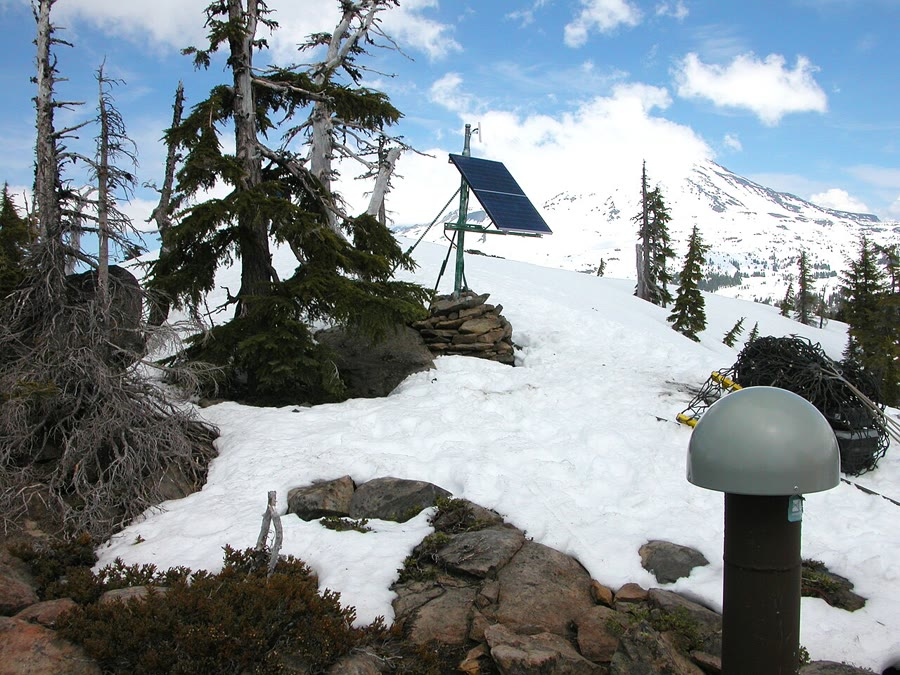
\includegraphics[width=0.62\linewidth]{images/book2/g11-usgs-gps-station.jpg}

{\small Uma estação permanente de posicionamento por satélite num vulcão da
Cordilheira das Cascatas, no Oregon (2007). A antena fica sob a cúpula
cinza, num mastro firmemente fincado no solo; o painel solar atrás alimenta
o receptor. Uma estação assim registra a sua própria posição dia após dia.
Fotografia: Dave Sherrod, USGS (domínio público).}
\end{omfigure}
% ledger: photo:g11-gps-station

\section{Placas rígidas sobre uma esfera}

Os terremotos não se espalham ao acaso pela Terra: quase todos acontecem ao
longo de faixas estreitas, os limites de placas (Livro 1, 7º ano). No
interior de uma placa, a rocha quase não se rompe. Uma placa, portanto, não
é uma pele mole que se estica e se enruga ao se mover, mas um pedaço rígido
de \omterm{def:g11:lithosphere-asthenosphere:lithosphere}{litosfera} que se move como um todo.

\begin{definition}[Placa rígida]\label{def:g11:plate-motions:rigid-plate}
Uma \emph{placa rígida}\index{placa rigida@placa rígida} é um pedaço de
\omterm{def:g11:lithosphere-asthenosphere:lithosphere}{litosfera} que se move como um único bloco: as distâncias entre os seus
pontos não mudam, e a sua deformação se concentra em zonas estreitas ao
longo dos seus limites.
\end{definition}

O modelo das \omterm{def:g11:plate-motions:rigid-plate}{placas rígidas} é uma aproximação. Algumas regiões se deformam
por centenas de quilômetros, como os planaltos altos atrás do Himalaia ou o
oeste da América do Norte, e o modelo as trata como limites largos. Mas,
sobre a maior parte da superfície da Terra, ele funciona notavelmente bem:
as velocidades que ele prevê para \omterm{def:g11:plate-motions:rigid-plate}{placas rígidas} coincidem com as que as
estações de satélite medem, com diferenças de poucos milímetros por ano
(\cref{sec:g11:plate-motions:predictive}), enquanto as placas se movem umas
em relação às outras a centímetros por ano.

Como uma calota rígida pode se mover sobre a superfície de uma esfera? Ela
não pode deslizar em linha reta, porque uma linha reta sai da esfera. Seja
qual for o movimento de uma calota rígida, ele é uma \emph{rotação} em torno
de um eixo que passa pelo centro da Terra. O eixo encontra a superfície no
\emph{polo de rotação} da placa. Um ponto da placa se move ao longo de um
pequeno círculo em torno desse polo, e quanto mais longe do polo ele fica,
maior o seu círculo e mais depressa ele se move (figura abaixo). A
demonstração de que todo movimento de uma calota rígida é uma rotação desse
tipo, e o uso dos polos de rotação para descrever os limites de placas,
ficam para o Livro~3; aqui, só as velocidades são usadas.

\begin{omfigure}
\begin{tikzpicture}[scale=1.15, font=\footnotesize]
  \fill[omSea!45] (0,0) circle (2);
  \draw (0,0) circle (2);
  % small circles about the rotation pole (pole at the top), seen slightly from above
  \foreach \a/\len in {60/0.75, 35/1.23, 0/1.5} {
    \pgfmathsetmacro{\r}{2*cos(\a)}
    \pgfmathsetmacro{\h}{2*sin(\a)}
    \draw[black!45, densely dashed] (-\r,\h) arc[start angle=180, end angle=0, x radius=\r, y radius=0.22*\r];
    \draw[omDef!80!black, line width=0.7pt] (-\r,\h) arc[start angle=180, end angle=360, x radius=\r, y radius=0.22*\r];
    \draw[-{Stealth[length=5pt]}, omProp, line width=1.1pt] (0,\h-0.22*\r) -- ++(\len,0);
  }
  \draw[black!70, dash pattern=on 3pt off 2pt] (0,-2.5) -- (0,2.55);
  \fill (0,2) circle (1.6pt);
  \node[anchor=south west] at (0.05,2.02) {polo de rotação};
  \node[anchor=north, text=black!70] at (0,-2.5) {eixo de rotação, pelo centro};
  \fill (0,0) circle (1pt);
  \node[anchor=west, align=left] at (2.25,0.9) {cada ponto se move\\ao longo de um pequeno\\círculo em torno do polo};
  \node[anchor=west, align=left, text=omProp] at (2.25,-0.4) {velocidade máxima\\a \ang{90} do polo};
\end{tikzpicture}

{\small Uma \omterm{def:g11:plate-motions:rigid-plate}{placa rígida} sobre uma esfera gira em torno de um eixo que passa
pelo centro da Terra. Os pontos perto do polo de rotação se movem devagar,
ao longo de pequenos círculos; os pontos a \ang{90} do polo se movem mais
depressa (setas: velocidades em escala).}
\end{omfigure}

A velocidade de um ponto é fácil de calcular. Um ponto a uma distância
angular $\theta$ do polo fica à distância $R\sin\theta$ do eixo, onde
$R = \qty{6371}{km}$ é o raio da Terra. Se a placa gira $\omega$
graus por milhão de anos, o ponto percorre em um milhão de anos a fração
$\omega/360$ do círculo de raio $R\sin\theta$:
\[
  v = \frac{\omega}{360} \times 2\pi R\sin\theta
    = \frac{\pi\,\omega}{180}\,R\sin\theta .
\]
Para $\omega = \qty{1}{\degree}$ por milhão de anos e $\theta = \ang{90}$,
isso dá $\pi \times 6371/180 \approx \qty{111}{km}$ por milhão de anos,
\qty{11.1}{cm} por ano. Uma placa não tem, portanto, uma única velocidade:
os seus pontos se movem a velocidades que vão de zero no polo de rotação (se
o polo fica sobre a placa) até um máximo a \ang{90} dele. As falhas
transformantes ao longo de uma dorsal, que deixam duas placas deslizarem uma
ao lado da outra, seguem pequenos círculos em torno do polo da rotação
relativa das duas placas.
% ledger: earth:Rmean (shared), nnr56:poles

Conjuntos publicados de polos de rotação dão, para cada placa, a posição do
seu polo e a sua taxa de rotação. Um deles, construído principalmente a
partir das taxas e das direções de expansão medidas ao longo das dorsais,
descreve 56 placas; a placa do Pacífico gira
\ang{0.651} por milhão de anos, a placa eurasiática \ang{0.223}. A partir
desses números, um computador calcula a velocidade de qualquer ponto de
qualquer placa (mapa abaixo).
% ledger: nnr56:poles, nnr56:data

\begin{omfigure}
\begin{tikzpicture}
\begin{axis}[ommap, width=\linewidth, xtick={-180,-90,...,180}, ytick={-60,0,60}]
\addplot[fill=omLithAlluv, draw=black!45, line width=0.2pt] table {figdata/out/shared-geo-land.dat};
\addplot[omRidge, line width=0.6pt] table {figdata/out/shared-geo-school-ridge.dat};
\addplot[omRidge!70!black, line width=0.6pt] table {figdata/out/shared-geo-school-transform.dat};
\addplot[omTrench, line width=0.6pt] table {figdata/out/shared-geo-school-subduction.dat};
\addplot[fill=omTrench, draw=none] table {figdata/out/shared-geo-school-teeth.dat};
\addplot[black!65, line width=0.6pt] table {figdata/out/shared-geo-school-collision.dat};
% computed in figdata/grade-11/plate_velocities.py (NNR-MORVEL56); 2.5 degrees per cm/yr
\addplot[black, line width=0.8pt, -{Stealth[length=4pt]}, quiver={u=\thisrow{dx}, v=\thisrow{dy}}]
  table[x=lon, y=lat] {figdata/out/grade-11-plate_velocities-arrows.dat};
\addplot[omProp, line width=1.2pt, -{Stealth[length=5pt]}, quiver={u=\thisrow{dx}, v=\thisrow{dy}}]
  table[x=lon, y=lat] {figdata/out/grade-11-plate_velocities-hawaii.dat};
\addplot[only marks, mark=*, mark size=1.3pt, omProp] coordinates {(-155.46,19.80)};
\node[font=\scriptsize, anchor=north, fill=white, fill opacity=0.75, text opacity=1, inner sep=1pt]
  at (axis cs:-150,15) {Mauna Kea};
\draw[black, line width=0.8pt, -{Stealth[length=4pt]}] (axis cs:-172,-80) -- (axis cs:-147,-80);
\node[font=\scriptsize, anchor=west, fill=white, fill opacity=0.75, text opacity=1, inner sep=1pt]
  at (axis cs:-145,-80) {\qty{10}{cm} por ano};
\end{axis}
\end{tikzpicture}

{\small As velocidades de pontos no interior de 16 placas, calculadas a
partir dos seus polos de rotação publicados, num referencial em que a
\omterm{def:g11:lithosphere-asthenosphere:lithosphere}{litosfera} como um todo não gira. As placas do Pacífico, de Nazca, de Cocos,
australiana e indiana se movem mais depressa; as placas eurasiática,
norte-americana, sul-americana e antártica, devagar. Seta vermelha: a placa
do Pacífico no Mauna Kea. Polos de rotação: Argus, Gordon e DeMets (2011);
limites de placas: Bird (2003); terras emersas: Natural Earth.}
\end{omfigure}
% ledger: nnr56:poles, data:pb2002, data:ne-land

\section{Medir os movimentos}

\subsection{Duas maneiras de medir uma velocidade}

As listras magnéticas do fundo do oceano dão a velocidade com que duas
placas se afastam através de uma dorsal (\cref{ch:g11:drift-to-spreading}):
divide-se a distância de uma listra até o eixo da dorsal pela sua idade. A
velocidade obtida é uma média sobre a idade da listra, muitas vezes os
últimos milhões de anos, e é uma velocidade \emph{relativa}, a de uma placa
vista da outra. As listras não dizem nada sobre placas que se encontram numa
fossa ou numa zona de colisão, já que ali não se forma fundo oceânico.

O posicionamento por satélite mede o movimento de um único ponto, hoje, ao
longo de alguns anos ou décadas. Uma estação permanente é ancorada na rocha
firme, de modo que se move com a placa; as suas posições diárias, em função
do tempo, se alinham ao longo de uma reta cuja inclinação é a velocidade da
estação.

\begin{method}[Uma taxa a partir de uma série temporal de posições]\label{met:g11:plate-motions:rate}
\begin{enumerate}
  \item Faça o gráfico da posição leste e da posição norte da estação em
        função do tempo, em dois gráficos ou no mesmo.
  \item Trace a reta que melhor acompanha cada série (ou leia nela dois
        pontos bem afastados). A sua inclinação, em milímetros por ano, é a
        velocidade leste $v_E$ ou a velocidade norte $v_N$; uma estação que
        se move para oeste ou para o sul tem velocidade negativa.
  \item A velocidade da estação é $v = \sqrt{v_E^2 + v_N^2}$; a sua direção
        faz com a linha leste--oeste o ângulo $\alpha$ tal que
        $\tan\alpha = |v_N|/|v_E|$, para o norte se $v_N > 0$ e para
        o leste se $v_E > 0$.
\end{enumerate}
\end{method}

\begin{omfigure}
\begin{tikzpicture}
\begin{axis}[ompt, name=a, width=0.5\linewidth, height=5.6cm, xmin=1995, xmax=2027, ymin=-200, ymax=120,
  xlabel={ano}, ylabel={posição (\unit{cm})}, xtick={2000,2010,2020},
  xticklabel style={/pgf/number format/set thousands separator={}},
  title={\small Mauna Kea, Havaí (MKEA)}, tick label style={font=\scriptsize}]
% computed in figdata/grade-11/gnss_series.py; ledger: data:b2-ngl-gnss
\addplot[only marks, mark=*, mark size=0.5pt, omDef] table[x=year, y=north] {figdata/out/grade-11-gnss_series-mkea.dat};
\addplot[only marks, mark=*, mark size=0.5pt, omProp] table[x=year, y=east] {figdata/out/grade-11-gnss_series-mkea.dat};
\node[font=\scriptsize, text=omDef!80!black, anchor=west] at (axis cs:1996.5,80) {norte};
\node[font=\scriptsize, text=omProp!80!black, anchor=west] at (axis cs:1996.5,-120) {leste};
\end{axis}
\begin{axis}[ompt, at={(a.east)}, anchor=west, xshift=0.9cm, width=0.5\linewidth, height=5.6cm, xmin=1995, xmax=2027,
  ymin=-10, ymax=70, xlabel={ano}, xtick={2000,2010,2020},
  xticklabel style={/pgf/number format/set thousands separator={}},
  title={\small Wettzell, Alemanha (WTZR)}, tick label style={font=\scriptsize}]
\addplot[only marks, mark=*, mark size=0.5pt, omDef] table[x=year, y=north] {figdata/out/grade-11-gnss_series-wtzr.dat};
\addplot[only marks, mark=*, mark size=0.5pt, omProp] table[x=year, y=east] {figdata/out/grade-11-gnss_series-wtzr.dat};
\node[font=\scriptsize, text=omDef!80!black, anchor=west] at (axis cs:2014,22) {norte};
\node[font=\scriptsize, text=omProp!80!black, anchor=west] at (axis cs:2006,40) {leste};
\end{axis}
\end{tikzpicture}

{\small Posições médias mensais de duas estações permanentes, medidas a
partir do seu primeiro mês: leste (vermelho) e norte (azul). Cada série se
alinha ao longo de uma reta, cuja inclinação é a velocidade da estação nessa direção. O Mauna Kea, na placa do Pacífico, se move para oeste e para o norte; Wettzell, na
placa eurasiática, para leste e para o norte, cerca de três vezes mais
devagar. Dados: Nevada Geodetic Laboratory (Blewitt, Hammond e Kreemer,
2018).}
\end{omfigure}
% ledger: data:b2-ngl-gnss

\begin{example}[A estação do Mauna Kea]\label{ex:g11:plate-motions:mkea}
De outubro de 1996 a setembro de 2026, as posições mensais da estação do
Mauna Kea seguem duas retas de inclinações $v_E =
\qty{-63.2}{mm}$ por ano (para oeste) e $v_N = \qty{+34.5}{mm}$ por ano. A
velocidade é $\sqrt{63.2^2 + 34.5^2} \approx \qty{72}{mm}$ por ano, e $\tan\alpha
= 34.5/63.2 \approx 0.546$ dá $\alpha \approx \ang{29}$: a estação se move
\qty{7.2}{cm} por ano numa direção \ang{29} ao norte do oeste. O polo de
rotação da placa do Pacífico prevê \qty{6.9}{cm} por ano, \ang{28} ao norte
do oeste, neste lugar.
\end{example}
% ledger: data:b2-ngl-gnss, nnr56:poles (prediction computed in plate_velocities.py)

Os pontos se dispersam alguns milímetros em torno das retas, muito menos que
o movimento de um único ano: depois de alguns anos de medição, a velocidade
de uma estação é conhecida com precisão melhor que um milímetro por ano.

\subsection{Movimento relativo e movimento absoluto}

Uma velocidade é sempre medida em relação a alguma coisa. A estação do Mauna
Kea se move \qty{7.2}{cm} por ano em relação a um referencial ligado à Terra
inteira; vista de uma estação na América do Norte, que também se move, a sua
velocidade é outra.

\begin{definition}[Movimento relativo; movimento absoluto]\label{def:g11:plate-motions:relative-motion}
O \emph{movimento relativo}\index{movimento relativo} de uma placa $A$ em
relação a uma placa $B$ é o seu movimento visto por um observador parado
sobre $B$. O \emph{movimento absoluto}\index{movimento absoluto} de uma
placa é o seu movimento em relação a um referencial ligado ao interior
profundo da Terra, por exemplo um conjunto de pontos quentes supostos fixos,
ou o referencial em que a \omterm{def:g11:lithosphere-asthenosphere:lithosphere}{litosfera} como um todo não gira.
\end{definition}

As dorsais, as fossas e as falhas transformantes são moldadas pelos
\omterm{def:g11:plate-motions:relative-motion}{movimentos relativos}: o que importa num limite é como as duas placas se
movem uma em relação à outra. As velocidades relativas se somam como os
deslocamentos que elas produzem.

\begin{proposition}[As velocidades relativas se somam como setas]\label{prop:g11:plate-motions:sum}
Seja $\vec v_{A/B}$ a velocidade da placa $A$ em relação à placa $B$, num
ponto dado do limite, e da mesma forma para os outros pares. Para quaisquer
três placas $A$, $B$, $C$,
\[
  \vec v_{A/C} = \vec v_{A/B} + \vec v_{B/C},
  \qquad\text{e}\qquad
  \vec v_{B/A} = -\vec v_{A/B}.
\]
\end{proposition}

\begin{proof}
Durante um curto intervalo $\Delta t$, um ponto fixo em $A$ vai da posição $P$
a $P'$, visto de $C$, e o ponto de $B$ que estava em $P$ vai a
$Q$, visto de $C$. Visto de $B$, o ponto de $A$ foi de $Q$ a
$P'$. Os deslocamentos se somam como vetores:
$\overrightarrow{PP'} = \overrightarrow{PQ} + \overrightarrow{QP'}$, isto é,
deslocamento de $A$ visto de $C$ = deslocamento de $B$ visto de $C$ +
deslocamento de $A$ visto de $B$. Dividindo por $\Delta t$, obtém-se $\vec v_{A/C}
= \vec v_{B/C} + \vec v_{A/B}$. Com $C = A$, o lado esquerdo é zero: $\vec
v_{B/A} = -\vec v_{A/B}$.
\end{proof}

\begin{method}[Fechar um triângulo de velocidades]\label{met:g11:plate-motions:triangle}
\begin{enumerate}
  \item Escreva cada velocidade conhecida com as suas componentes leste e
        norte, todas medidas no mesmo ponto.
  \item Para encontrar $\vec v_{A/B}$ a partir das velocidades de $A$ e de
        $B$ num mesmo referencial $C$, subtraia: $\vec v_{A/B} = \vec v_{A/C} - \vec v_{B/C}$,
        componente por componente.
  \item Num desenho, coloque as origens de $\vec v_{A/C}$ e de $\vec v_{B/C}$
        no mesmo ponto: a seta que vai da ponta de $\vec v_{B/C}$ à ponta de
        $\vec v_{A/C}$ é $\vec v_{A/B}$, e ela fecha o triângulo.
  \item Calcule o seu comprimento e a sua direção como no
        \cref{met:g11:plate-motions:rate}.
\end{enumerate}
\end{method}

\begin{example}[A falha de San Andreas]\label{ex:g11:plate-motions:san-andreas}
No centro da Califórnia, a \ang{35.5} Norte e \ang{120.5} Oeste, os polos de
rotação dão à placa do Pacífico a velocidade $(-42.1, +26.4)$ e à placa
norte-americana $(-11.9, -14.8)$, em milímetros por ano (leste, norte), no
referencial da \omterm{def:g11:lithosphere-asthenosphere:lithosphere}{litosfera} inteira. A placa do Pacífico em relação à América
do Norte se move a $(-42.1 + 11.9,\ 26.4 + 14.8) = (-30.2, +41.2)$, isto é,
$\sqrt{30.2^2 + 41.2^2} \approx \qty{51}{mm}$ por ano, numa direção
\ang{36} a oeste do norte (figura abaixo). A falha
de San Andreas, que corre para noroeste, absorve a maior parte desse
deslizamento.
\end{example}
% ledger: nnr56:poles (computed in plate_velocities.py: relative pa/na at 120.5 W 35.5 N)

\begin{omfigure}
\begin{tikzpicture}[x=0.065cm, y=0.065cm, font=\footnotesize]
  % mm/yr, from plate_velocities.py: PA (-42.1, 26.4), NA (-11.9, -14.8), PA/NA (-30.2, 41.2)
  \draw[black!25] (-8,0) -- (8,0) (0,-8) -- (0,8);
  \draw[-{Stealth[length=5pt]}, omProp, line width=1.1pt] (0,0) -- (-42.1,26.4)
    node[pos=0.55, above right, inner sep=1pt] {$\vec v_{\mathrm{PA}}$};
  \draw[-{Stealth[length=5pt]}, omDef, line width=1.1pt] (0,0) -- (-11.9,-14.8)
    node[pos=0.8, right=2pt] {$\vec v_{\mathrm{NA}}$};
  \draw[-{Stealth[length=5pt]}, black, line width=1.1pt] (-11.9,-14.8) -- (-42.1,26.4)
    node[pos=0.4, left=9pt, align=right] {$\vec v_{\mathrm{PA/NA}}$\\\qty{51}{mm} por ano};
  \fill (0,0) circle (0.9pt);
  % compass
  \draw[-{Stealth[length=4pt]}] (25,10) -- (25,24) node[above] {N};
  \draw[-{Stealth[length=4pt]}] (25,10) -- (39,10) node[right] {L};
  \draw (25,-18) -- (40.4,-18);
  \node[below] at (32.7,-18) {\qty{20}{mm} por ano};
  \draw (25,-17) -- (25,-19) (40.4,-17) -- (40.4,-19);
\end{tikzpicture}

{\small Fechar um triângulo de velocidades no centro da Califórnia (em
escala). Vermelho: a placa do Pacífico; azul: a placa norte-americana, ambas
no referencial da \omterm{def:g11:lithosphere-asthenosphere:lithosphere}{litosfera} inteira. Preto: a placa do Pacífico vista da
América do Norte, a seta que vai da ponta da azul à ponta da vermelha.}
\end{omfigure}

\section{Rastros de pontos quentes}

\subsection{Uma placa sobre uma pluma fixa}

O Havaí fica no meio da placa do Pacífico, a mais de \qty{3000}{km} do
limite de placa mais próximo.
% ledger: usgs:hawaii-hotspot (Book 1 row)
 Os seus vulcões são alimentados por um ponto quente (Livro~1,
7º~ano). A placa se move sobre ele, e cada vulcão é levado para longe do
ponto quente enquanto um novo cresce atrás dele.

\begin{definition}[Rastro de ponto quente]\label{def:g11:plate-motions:hotspot-track}
Um \emph{rastro de ponto quente}\index{rastro de ponto quente} é a linha de
vulcões, e de vulcões submersos chamados montes submarinos, que uma placa
leva para longe de um ponto quente ao se mover sobre ele: o vulcão ativo
fica sobre o ponto quente, e os vulcões são cada vez mais antigos com a
distância a ele.
\end{definition}

\begin{omfigure}
\begin{tikzpicture}[font=\footnotesize]
  % plate moving to the left over a fixed plume (not to scale)
  \fill[omSea!50] (0,0) rectangle (11,0.9);
  \fill[black!22] (0,-0.9) rectangle (11,0);
  \draw (0,0) -- (11,0);
  \draw[densely dashed] (0,0.9) -- (11,0.9) node[right] {nível do mar};
  \node[anchor=east] at (10.95,-0.45) {litosfera};
  \fill[omLithPeridotite!40] (0,-2.3) rectangle (11,-0.9);
  \node[anchor=west] at (0.1,-1.6) {astenosfera};
  % plume
  \fill[omProp!55] (8.6,-2.3) -- (8.6,-1.2) .. controls (8.6,-0.9) and (9.2,-0.9) .. (9.2,-1.2) -- (9.2,-2.3) -- cycle;
  \fill[omProp!55] (8.75,-0.95) rectangle (9.05,0);
  \node[anchor=north, align=center] at (8.9,-2.35) {pluma, fixa no manto};
  % volcanoes: active over the plume, older ones carried left, eroded and sunk
  \fill[black!65] (8.0,0) -- (8.9,1.6) -- (9.8,0) -- cycle;
  \fill[black!55] (5.4,0) -- (6.2,1.15) -- (7.0,0) -- cycle;
  \fill[black!50] (3.0,0) -- (3.55,0.62) -- (3.85,0.62) -- (4.4,0) -- cycle;
  \fill[black!45] (0.8,0) -- (1.25,0.42) -- (1.65,0.42) -- (2.1,0) -- cycle;
  \node[above] at (8.9,1.6) {ativo};
  \node[above] at (6.2,1.15) {$t_1$};
  \node[above] at (3.7,0.62) {$t_2$};
  \node[above] at (1.45,0.42) {$t_3$};
  % plate motion
  \draw[-{Stealth[length=6pt]}, line width=1.2pt] (6.5,-0.45) -- (4.0,-0.45) node[left] {a placa se move, velocidade $v$};
  % distance d = v t
  \draw[{Stealth[length=4pt]}-{Stealth[length=4pt]}] (3.7,2.3) -- (8.9,2.3) node[midway, above] {$d_2 = v\,t_2$};
  \draw[black!50] (3.7,1.05) -- (3.7,2.4) (8.9,2.0) -- (8.9,2.4);
\end{tikzpicture}

{\small Uma placa que se move à velocidade $v$ sobre uma pluma fixa no manto
(fora de escala). Um vulcão de idade $t$, construído sobre a pluma, foi
levado à distância $d = v\,t$; os vulcões mais antigos são erodidos e
afundam abaixo do mar.}
\end{omfigure}

\begin{proposition}[Velocidade a partir de um rastro de ponto quente]\label{prop:g11:plate-motions:hotspot}
Se um ponto quente fica fixo no manto profundo e a placa acima dele se move
a uma velocidade constante $v$ numa direção constante, um vulcão que estava
sobre o ponto quente há um tempo $t$ fica agora à distância
\[
  d = v\,t
\]
do vulcão ativo, ao longo do rastro. As idades dos vulcões, em função das
suas distâncias, caem numa reta que passa pela origem, de inclinação $1/v$,
e $v$ é a velocidade absoluta da placa.
\end{proposition}

\begin{proof}
O vulcão foi construído onde a placa estava sobre o ponto quente, e desde
então se move com a placa. Durante o tempo $t$, a placa se deslocou
$v\,t$ numa direção fixa, de modo que o vulcão fica a essa distância do
ponto da placa que agora está sobre o ponto quente, onde fica o vulcão
ativo. A relação $t = d/v$ é a de uma reta que passa pela origem, de
inclinação $1/v$. A velocidade é medida em relação ao ponto quente, isto é,
em relação ao manto profundo: é uma velocidade absoluta.
\end{proof}

\subsection{A cadeia Havaí--Imperador}

A partir da ilha do Havaí, uma linha de ilhas, recifes e montes submarinos
se estende por uns \qty{3400}{km} para oés-noroeste, depois vira bruscamente
e continua para o norte como os montes submarinos do Imperador, o monte
submarino Suiko, sozinho, ficando a \qty{4860}{km} do Kilauea, até as
fossas ao largo de Kamchatka e das Aleutas (imagem abaixo).
% ledger: cd87:ages

\begin{omfigure}
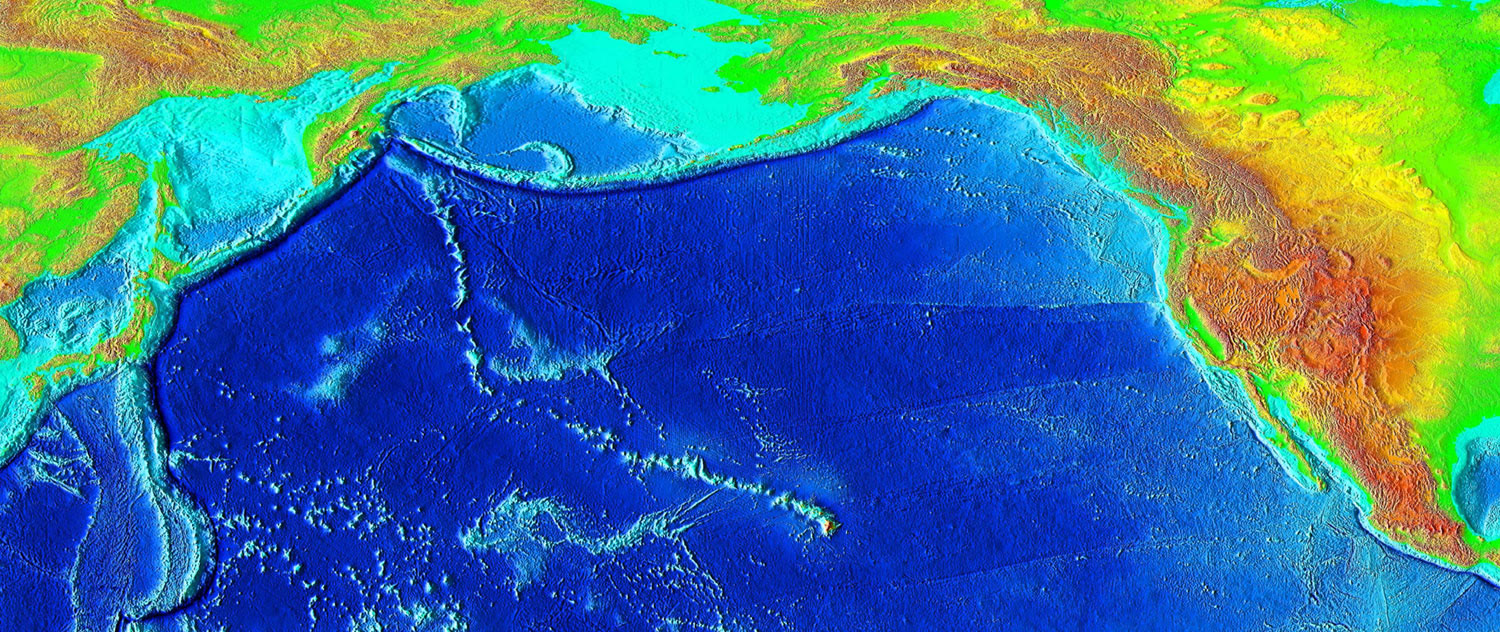
\includegraphics[width=\linewidth]{images/book2/g11-ngdc-hawaii-chain.jpg}

{\small Relevo sombreado do fundo do Pacífico Norte. A cadeia havaiana vai
da ilha do Havaí (embaixo, no centro, em marrom) para oés-noroeste; na
curva, ela vira para o norte nos montes submarinos do Imperador, que
terminam na fossa ao longo de Kamchatka e das Aleutas. Imagem: National
Geophysical Data Center, NOAA (domínio público).}
\end{omfigure}
% ledger: photo:g11-hawaii-chain

A datação potássio--argônio de lavas de 37 vulcões da cadeia, coletadas nas
ilhas, dragadas dos montes submarinos ou obtidas por perfuração através dos
seus sedimentos, dá as suas idades (gráfico abaixo). O Mauna Kea tem cerca
de \num{0.4} milhão de anos, Kauai \num{5.1}, Midway \num{27.7}, e o
monte submarino Suiko, perto da extremidade da cadeia do Imperador,
\num{64.7}. As idades crescem com a distância ao Kilauea, o vulcão ativo,
como prevê um \omterm{def:g11:plate-motions:hotspot-track}{rastro de ponto quente}.
% ledger: cd87:ages

\begin{omfigure}
\begin{tikzpicture}
\begin{axis}[ompt, width=0.82\linewidth, height=6.4cm, xmin=0, xmax=5000, ymin=0, ymax=70,
  xlabel={distância ao Kilauea ao longo da cadeia (\unit{km})}, ylabel={idade (milhões de anos)},
  xticklabel style={/pgf/number format/set thousands separator={}},
  legend style={font=\scriptsize, at={(0.03,0.97)}, anchor=north west}, legend cell align=left]
% computed in figdata/grade-11/hawaii_chain.py; ledger: cd87:ages
\addplot[only marks, mark=o, mark size=1.6pt, omDef, error bars/.cd, y dir=both, y explicit]
  table[x=dist, y=age, y error=err] {figdata/out/grade-11-hawaii_chain-hawaiian.dat};
\addplot[only marks, mark=triangle, mark size=2pt, omProp, error bars/.cd, y dir=both, y explicit]
  table[x=dist, y=age, y error=err] {figdata/out/grade-11-hawaii_chain-emperor.dat};
\addplot[black, densely dashed, line width=0.6pt] table[x=dist, y=age] {figdata/out/grade-11-hawaii_chain-fit.dat};
\legend{cadeia havaiana, curva e cadeia do Imperador, {reta pela origem, \qty{9.1}{cm} por ano}}
\draw[black!50, densely dotted] (axis cs:3400,0) -- (axis cs:3400,70);
\node[font=\scriptsize, anchor=south, rotate=90] at (axis cs:3400,8) {curva};
\node[font=\scriptsize, anchor=north west] at (axis cs:519,5.1) {Kauai};
\node[font=\scriptsize, anchor=south] at (axis cs:2432,30) {Midway};
\node[font=\scriptsize, anchor=south east] at (axis cs:4860,65.5) {Suiko};
\end{axis}
\end{tikzpicture}

{\small Idade dos vulcões da cadeia Havaí--Imperador em função da sua
distância ao Kilauea, com as incertezas das idades. Ao longo da cadeia
havaiana, os pontos seguem uma reta que passa pela origem; além da curva, as
idades crescem mais depressa com a distância. Dados: Clague e Dalrymple
(1987).}
\end{omfigure}

Ao longo da cadeia havaiana, até cerca de \qty{3300}{km}, os pontos se
dispersam em torno de uma reta que passa pela origem. A reta que melhor se
ajusta aos 26 vulcões datados dessa parte sobe um milhão de anos a cada
\qty{91}{km}: pela \cref{prop:g11:plate-motions:hotspot}, a placa do
Pacífico se moveu sobre o ponto quente a cerca de \qty{91}{km} por milhão de
anos, \qty{9.1}{cm} por ano. Os autores das idades, ajustando a cadeia
inteira à sua maneira, encontraram \qty{8.6}{cm} por ano.
% ledger: cd87:ages (fit computed in hawaii_chain.py), cd87:rate

Além da curva, as idades crescem mais depressa com a distância: ao longo da
cadeia do Imperador, a placa se moveu mais devagar, cerca de \qty{6.5}{cm}
por ano em média (melhor reta pelos nove montes submarinos datados). E a
cadeia muda de direção. Se o ponto quente ficou no lugar, a curva registra
uma mudança na direção do movimento da placa do Pacífico. Idades mais
recentes situam o início da curva perto do monte submarino Kimmei, há cerca
de 50 milhões de anos, ao mesmo tempo que uma reorganização das dorsais do
Pacífico e os primeiros vulcões dos arcos insulares ao longo da sua borda
oeste: a placa mudou de rumo.
% ledger: cd87:ages (Emperor fit computed in hawaii_chain.py), sc06:bend

\section{O poder de previsão do modelo}\label{sec:g11:plate-motions:predictive}

O modelo das placas diz que algumas \omterm{def:g11:plate-motions:rigid-plate}{placas rígidas} giram em torno dos seus
polos de rotação, e que quase tudo acontece nos seus limites. A sua força
está em que medições feitas por métodos inteiramente diferentes, ao longo de
intervalos de tempo muito diferentes, dão as mesmas respostas.

\begin{itemize}
  \item \emph{Os terremotos e os vulcões} se concentram ao longo dos limites,
        e o tipo de limite prevê o seu tipo: terremotos rasos ao longo das
        dorsais, profundos apenas perto das fossas (\cref{ch:g11:subduction-zones}).
  \item \emph{O fundo do oceano} é mais jovem ao longo das dorsais e cada vez
        mais antigo longe delas, simetricamente dos dois lados
        (\cref{ch:g11:drift-to-spreading}).
  \item \emph{As cadeias de montanhas} se erguem onde as placas convergem: a
        Índia ainda se move em direção à Eurásia a cerca de \qty{4.5}{cm} por
        ano através do Himalaia, como calculado a partir dos polos de rotação
        (\cref{ch:g12:mountain-building}).
  \item \emph{As velocidades concordam entre os métodos}: a tabela abaixo
        compara as velocidades medidas hoje por posicionamento por satélite
        com as previstas pelos polos de rotação, cujas \omterm{def:g11:drift-to-spreading:spreading-rate}{taxas de expansão} vêm
        principalmente das listras magnéticas e fazem a média do movimento
        nos últimos \num{0.8} a \num{3.2} milhões de anos, e com a velocidade
        registrada por um \omterm{def:g11:plate-motions:hotspot-track}{rastro de ponto quente} ao longo de dezenas de
        milhões de anos.
\end{itemize}
% ledger: nnr56:poles, nnr56:data (India-Eurasia computed in plate_velocities.py at 85 E 28 N)

\begin{center}
\small
\begin{tabular}{|l|c|c|}
\hline
o que é medido & método & velocidade (\unit{cm}/ano) \\ \hline
Mauna Kea, placa do Pacífico & posicionamento por satélite, 30 anos & 7.2 \\
Mauna Kea, placa do Pacífico & polo de rotação & 6.9 \\
Wettzell, placa eurasiática & posicionamento por satélite, 31 anos & 2.6 \\
Wettzell, placa eurasiática & polo de rotação & 2.3 \\
Pacífico, sobre o ponto quente do Havaí & idade dos vulcões, 40 milhões de anos & 9.1 \\ \hline
\end{tabular}
\end{center}
% ledger: data:b2-ngl-gnss, nnr56:poles, cd87:ages (all computed in figdata/grade-11)

As velocidades dos polos de rotação e as das estações concordam com
diferença de até \qty{0.3}{cm} por ano, embora as primeiras sejam médias de
milhões de anos e as segundas, de apenas décadas: as placas se movem hoje
como se moveram durante milhões de anos. A velocidade do ponto quente é
maior: ela é medida em outro referencial, o do próprio ponto quente, e ao
longo de um tempo muito mais longo.

Mais um padrão aparece quando se comparam as velocidades de placas
inteiras. As placas que se movem mais depressa, Cocos, Nazca, Pacífico,
australiana e filipina, têm todas uma longa borda que afunda no manto numa
fossa; as suas velocidades médias ficam em torno de \qty{6.5}{cm} por ano.
As placas sem uma borda desse tipo, entre elas as placas eurasiática,
norte-americana, sul-americana, africana e antártica, se movem a cerca de
\qty{2.4}{cm} por ano em média. Essa pista sobre o que move as placas é
retomada no \cref{ch:g11:subduction-zones}.
% ledger: nnr56:rms (means computed in plate_velocities.py)

\section{Exercícios}

\begin{exercise}[$\star$]\label{exo:g11:plate-motions:1}
Defina uma \omterm{def:g11:plate-motions:rigid-plate}{placa rígida}. Onde se concentra a deformação da \omterm{def:g11:lithosphere-asthenosphere:lithosphere}{litosfera}, e que
observação sísmica corriqueira mostra isso?
\end{exercise}

\begin{exercise}[$\star$]\label{exo:g11:plate-motions:2}
A estação do Mauna Kea se move \qty{72}{mm} por ano. Expresse essa
velocidade em quilômetros por milhão de anos. Quanto a estação se desloca em
30 anos? E em um milhão de anos?
\end{exercise}

\begin{exercise}[$\star$]\label{exo:g11:plate-motions:3}
Em dez anos, uma estação se deslocou \qty{30}{cm} para leste e \qty{40}{cm}
para o norte. Encontre as suas velocidades leste e norte, a sua velocidade e
o ângulo que a sua direção faz com o norte.
\end{exercise}

\begin{exercise}[$\star$]\label{exo:g11:plate-motions:4}
Defina um \omterm{def:g11:plate-motions:hotspot-track}{rastro de ponto quente}. Ao longo da cadeia havaiana, onde fica o
vulcão mais jovem, e em que direção as idades aumentam? O que isso diz sobre
a direção em que a placa do Pacífico se move?
\end{exercise}

\begin{exercise}[$\star$]\label{exo:g11:plate-motions:5}
Kauai fica a \qty{519}{km} do Kilauea ao longo da cadeia, e as suas lavas
mais antigas têm \num{5.1} milhões de anos. Supondo o ponto quente fixo, a
que velocidade média a placa a transportou, em quilômetros por milhão de
anos e em centímetros por ano?
\end{exercise}

\begin{exercise}[$\star\star$]\label{exo:g11:plate-motions:6}
No gráfico das séries das duas estações, a estação de Wettzell se deslocou
cerca de \qty{63}{cm} para leste e \qty{48}{cm} para o norte em 31 anos.
Encontre as suas velocidades leste e norte, a sua velocidade e a sua
direção. Compare a sua velocidade com a do Mauna Kea.
\end{exercise}

\begin{exercise}[$\star\star$]\label{exo:g11:plate-motions:7}
Na Islândia, a \ang{64.5} Norte e \ang{18} Oeste, os polos de rotação dão à
placa norte-americana a velocidade $(-10.5, +20.6)$ e à placa eurasiática
$(+7.7, +16.3)$, em milímetros por ano (leste, norte). (1) Encontre a
velocidade da América do Norte em relação à Eurásia, a sua velocidade
escalar e a sua direção. (2) O que é essa velocidade para a dorsal que
atravessa a Islândia? (3) Compare com a taxa de \qty{2}{cm} por ano muitas
vezes citada para o Atlântico Norte.
\end{exercise}

\begin{exercise}[$\star\star$]\label{exo:g11:plate-motions:8}
A placa do Pacífico gira \ang{0.651} por milhão de anos. (1) Encontre a
velocidade de um ponto a \ang{90} do seu polo de rotação, em centímetros por
ano. (2) E a de um ponto a \ang{30} do polo? (3) Em que lugar de uma placa a
velocidade é zero? A velocidade de uma placa inteira pode ser dada por um
único número?
\end{exercise}

\begin{exercise}[$\star\star$]\label{exo:g11:plate-motions:9}
Ao norte do Himalaia, a \ang{28} Norte e \ang{85} Leste, os polos de
rotação dão à placa indiana a velocidade $(+40.6, +38.6)$ e à placa
eurasiática $(+24.0, -3.3)$, em milímetros por ano (leste, norte).
(1) Encontre a velocidade da Índia em relação à Eurásia, a sua velocidade
escalar e a sua direção. (2) Se ela não mudasse, quanto as duas placas
convergiriam em 10 milhões de anos?
\end{exercise}

\begin{exercise}[$\star\star$]\label{exo:g11:plate-motions:10}
Necker fica a \qty{1058}{km} do Kilauea e tem \num{10.3} milhões de anos;
Midway fica a \qty{2432}{km} e tem \num{27.7} milhões de anos. Encontre a
velocidade da placa sobre o ponto quente entre as épocas em que os dois
vulcões foram construídos. Compare com \qty{9.1}{cm} por ano.
\end{exercise}

\begin{exercise}[$\star\star$]\label{exo:g11:plate-motions:11}
Num ponto, a placa $A$ se move \qty{3}{cm} por ano para leste em relação à
placa $B$, e a placa $B$ se move \qty{4}{cm} por ano para o norte em relação
à placa $C$. (1) Desenhe o triângulo de velocidades e encontre a velocidade
de $A$ em relação a $C$: velocidade escalar e direção. (2) Qual é a
velocidade de $C$ em relação a $A$?
\end{exercise}

\begin{exercise}[$\star\star\star$]\label{exo:g11:plate-motions:12}
O Mauna Kea fica a \qty{54}{km} do Kilauea e tem \num{0.375} milhão de anos.
(1) Que velocidade ele dá para a placa? (2) Um vulcão tem algumas dezenas de
quilômetros de diâmetro, e cresce durante várias centenas de milhares de
anos. Suponha que a sua distância ao ponto quente seja incerta em
\qty{25}{km}: entre que valores fica então a velocidade? (3) Explique por
que os vulcões jovens, perto do ponto quente, dão uma estimativa ruim da
velocidade, e por que os vulcões longe dele são melhores.
\end{exercise}

\begin{exercise}[$\star\star\star$]\label{exo:g11:plate-motions:13}
As posições mensais de uma estação se dispersam cerca de \qty{5}{mm} em
torno da sua reta. Um movimento é visto com clareza quando passa de dez
vezes a dispersão. (1) Por quanto tempo é preciso medir para ver com clareza
o movimento da estação do Mauna Kea, \qty{72}{mm} por ano? (2) E um
movimento de \qty{5}{mm} por ano, como através de uma região que se deforma
lentamente no interior de um continente? (3) Por que as velocidades das
placas foram medidas pelas listras magnéticas muito antes que os satélites
pudessem medi-las?
\end{exercise}

\begin{exercise}[$\star\star\star$]\label{exo:g11:plate-motions:14}
Na Dorsal Mesoatlântica a \ang{30} Sul (\ang{13.5} Oeste), os polos de
rotação dão à placa sul-americana a velocidade $(-4.9, +11.0)$ e à placa
africana $(+27.1, +17.9)$, em milímetros por ano (leste, norte).
(1) Encontre a velocidade da América do Sul em relação à África, a sua
velocidade escalar e a sua direção. (2) Deduza a \omterm{def:g11:drift-to-spreading:spreading-rate}{taxa de expansão total} e a
\omterm{def:g11:drift-to-spreading:spreading-rate}{semitaxa de expansão} da dorsal. (3) Os sedimentos do Atlântico Sul deram
uma semitaxa de cerca de \qty{1.9}{cm} por ano, em média nos últimos 66
milhões de anos (\cref{ch:g11:drift-to-spreading}). Compare, e sugira o que a
diferença pode significar.
\end{exercise}

\begin{exercise}[$\star\star\star$]\label{exo:g11:plate-motions:15}
Uma estação se move de forma constante \qty{20}{mm} por ano para leste.
Exatamente na metade de dez anos de medição, um terremoto a desloca de
repente \qty{50}{mm} para oeste. (1) Esboce a sua posição leste em função do
tempo. (2) Que velocidade se encontraria apenas com a primeira e a última
posições? (3) Que velocidade dá cada metade da série, sozinha? (4) Como um
geodesista deve tratar um salto desse tipo?
\end{exercise}

\section{Problema: ler a cadeia Havaí--Imperador}

\begin{problem}[{Problema de fim de semana --- a velocidade de uma placa escrita em vulcões}]
\label{pb:g11:plate-motions:1}
% values from Clague and Dalrymple 1987, Table 1.4 (ledger cd87:ages); fits computed in
% figdata/grade-11/hawaii_chain.py (v_hawaiian 91.2, v_emperor_free 64.6); bend sc06:bend;
% MKEA rates data:b2-ngl-gnss
A tabela dá a distância ao Kilauea, medida ao longo da cadeia, e a idade
potássio--argônio de treze vulcões da cadeia Havaí--Imperador. O Kilauea é
o vulcão ativo sobre o ponto quente; a curva fica entre Abbott e
Daikakuji.

\begin{center}
\small
\begin{tabular}{|l|c|c||l|c|c|}
\hline
vulcão & distância (\unit{km}) & idade (\unit{Ma}) & vulcão & distância (\unit{km}) & idade (\unit{Ma}) \\ \hline
Mauna Kea & 54 & 0.375 & Abbott & 3280 & 38.7 \\ \hline
Kauai & 519 & 5.1 & Daikakuji & 3493 & 42.4 \\ \hline
Nihoa & 780 & 7.2 & Koko (sul) & 3758 & 48.1 \\ \hline
Necker & 1058 & 10.3 & Ojin & 4102 & 55.2 \\ \hline
Laysan & 1818 & 19.9 & Nintoku & 4452 & 56.2 \\ \hline
Midway & 2432 & 27.7 & Suiko (centro) & 4860 & 64.7 \\ \hline
Colahan & 3128 & 38.6 & & & \\ \hline
\end{tabular}
\end{center}

\medskip
\noindent\textbf{Parte I --- Idades e distâncias.}
\begin{enumerate}
  \item Que vulcão da tabela é o mais jovem, e qual é o mais antigo? Como as
        idades mudam ao longo da cadeia?
  \item Mostre que uma distância em quilômetros dividida por uma idade em
        milhões de anos é uma velocidade em milímetros por ano.
  \item Calcule a velocidade média $d/t$ dada por Kauai.
  \item Calcule $d/t$ para Necker, Laysan, Midway, Colahan e Abbott.
  \item Faça o gráfico da idade em função da distância para os oito vulcões
        da tabela que ficam antes da curva. Os pontos ficam perto de uma reta que passa
        pela origem?
\end{enumerate}

\medskip
\noindent\textbf{Parte II --- A velocidade da placa sobre o ponto quente.}
\begin{enumerate}[resume]
  \item Explique por que, para um ponto quente fixo e uma placa que se move
        a uma velocidade constante $v$, a idade $t$ e a distância $d$
        satisfazem $t = d/v$.
  \item Calcule a média das cinco velocidades da questão~4.
  \item A reta que passa pela origem e melhor se ajusta a todos os 26
        vulcões datados da cadeia havaiana dá \qty{91}{km} por milhão de
        anos. Compare com a questão~7.
  \item A essa velocidade, quanto tempo a placa levaria para levar Kauai do
        ponto quente até o seu lugar atual? Compare com a sua idade.
  \item Em que direção a placa do Pacífico se move sobre o ponto quente?
\end{enumerate}

\medskip
\noindent\textbf{Parte III --- A curva.}
\begin{enumerate}[resume]
  \item Calcule a velocidade média da placa entre as épocas em que Daikakuji
        e Suiko (centro) foram construídos.
  \item A melhor reta pelos nove vulcões datados a partir de Daikakuji dá
        \qty{65}{km} por milhão de anos. Compare com a velocidade ao longo
        da cadeia havaiana.
  \item Idades mais recentes situam o início da curva perto do monte
        submarino Kimmei, a \qty{3668}{km} do Kilauea, há cerca de 50
        milhões de anos. Que velocidade média isso dá para a cadeia havaiana
        inteira? Compare com \qty{91}{km} por milhão de anos, e explique por
        que os dois podem estar certos.
  \item Se o ponto quente ficou fixo, o que a curva registra sobre a placa
        do Pacífico?
  \item A datação mais recente encontrou grandes mudanças de velocidade ao
        longo da cadeia do Imperador, com pouca mudança na sua direção.
        Explique por que a direção de uma cadeia e o espaçamento das suas
        idades são duas informações independentes.
\end{enumerate}

\medskip
\noindent\textbf{Parte IV --- Comparação com a medição atual por satélite.}
\begin{enumerate}[resume]
  \item A estação do Mauna Kea se move $\qty{-63.2}{mm}$ por ano para leste
        e $\qty{+34.5}{mm}$ por ano para o norte. Encontre a sua velocidade e
        a sua direção.
  \item A cadeia havaiana vai do Kilauea para oés-noroeste. A direção da
        estação é compatível com ela?
  \item A estação dá \qty{7.2}{cm} por ano, a cadeia \qty{9.1}{cm} por ano.
        Dê duas razões pelas quais os dois números não precisam ser iguais.
  \item A \qty{91}{km} por milhão de anos, quanto tempo a placa levará para
        levar o Mauna Kea mais \qty{100}{km} para longe do ponto quente?
  \item Conclua: a que velocidade a placa do Pacífico se moveu sobre o ponto
        quente do Havaí durante os últimos 40 milhões de anos?
\end{enumerate}
\end{problem}
